\chapter{Metodologia}

\section{Tipo de pesquisa}

O presente estudo caracteriza-se como pesquisa aplicada, de natureza tecnológica e abordagem mista. Foram combinadas técnicas qualitativas e quantitativas, como levantamento documental e estudo de caso único, com foco na plataforma Pró-Mamá e seus serviços \emph{web} (\emph{API} e painel administrativo). O aplicativo móvel, embora relacionado, não constitui objeto central por ser resultado de outro trabalho acadêmico.

O delineamento temporal do estudo foi estruturado em três fases: diagnóstico, reconstrução e validação. Na primeira fase, foram coletados documentos internos e registros históricos, incluindo versões de código, relatórios de implantação, problemas e requisitos originais. Também foi realizado levantamento de aplicativos de saúde digital, considerando funcionalidades, integrações e políticas de dados, a fim de estabelecer parâmetros de comparação para a conjuntura do Pró-Mamá.

\section{Levantamento documental}

A etapa de levantamento documental assumiu caráter exploratório, buscando identificar práticas em ecossistemas de saúde digital. Inicialmente, foram analisados aplicativos móveis de aleitamento materno disponíveis nas lojas \emph{Google Play} e na \emph{App Store}. O objetivo foi mapear decisões técnicas e regras de negócio associadas. Foram enviados questionários a cinquenta equipes desenvolvedoras, porém não houve retorno, o que representou uma limitação metodológica e motivou a ampliação do escopo da investigação.

A ampliação considerou aplicações relacionadas à gestação e ao cuidado infantil, desde que apresentassem documentação acessível ou outras formas de análise além da observação direta no aplicativo. Essa decisão metodológica visou garantir maior comparabilidade entre os sistemas analisados e os objetos de estudo desta pesquisa.

Essa estratégia permitiu uma análise mais abrangente, tornando-se possível observar tendências e práticas consolidadas em soluções digitais de saúde. A análise dos resultados será detalhada no capítulo de \hyperref[cap_trabalhos_relacionados]{Trabalhos Relacionados}.

\section{Metodologia de desenvolvimento}

As metodologias ágeis surgiram como uma resposta às limitações dos modelos tradicionais de desenvolvimento, propondo maior flexibilidade, adaptação às mudanças e entregas frequentes de valor ao usuário. De acordo com \citeonline{NagaiSbragia2023Agil}, a consolidação dessas práticas está associada à priorização da colaboração, da comunicação contínua e da entrega incremental de resultados, fatores cruciais em ambientes complexos e em constante transformação.

Entre os métodos ágeis, o modelo incremental destaca-se pela entrega em etapas sucessivas. Como destacam \citeonline{Lima2023IncrementalModel}, “o modelo incremental é uma metodologia ágil e iterativa que possibilita a entrega de resultados em etapas e em um curto espaço de tempo, permitindo que os clientes monitorem atentamente o progresso do projeto e realizem ajustes ou alterações, se necessário”. Essa característica favorece maior controle de qualidade e mitigação de riscos.

No caso do Pró-Mamá, a reconstrução da plataforma foi planejada em pequenos incrementos, permitindo validação contínua pelos profissionais de saúde. Cada funcionalidade previamente definida foi fragmentada em partes menores, implementadas, testadas e revisadas em ciclos curtos. Essa abordagem garantiu maior aderência às necessidades reais dos usuários e possibilitou a incorporação de \emph{feedbacks} ao longo do processo.

\section{Análise e (re)especificação de requisitos}

A engenharia de requisitos é o processo que visa compreender e documentar o que o sistema deve realizar, sendo considerada uma das atividades mais críticas dentro da engenharia de \emph{software}. Como define \citeonline{sommerville2011engenharia}, trata-se da “atividade de descobrir, analisar, documentar e verificar os serviços e restrições do sistema”. Nesse cenário, a análise de requisitos busca transformar necessidades dos usuários e restrições de negócio em especificações claras e compreensíveis.

Segundo \citeonline{sommerville2011engenharia}, “a falha em compreender as reais necessidades dos usuários está entre as principais causas de insucesso de projetos de \emph{software}, tornando essencial o uso de boas práticas e técnicas de elicitação para reduzir ambiguidades e conflitos”. Essa afirmação destaca a relevância de aplicar métodos estruturados na análise de requisitos, garantindo maior qualidade e confiabilidade ao processo de desenvolvimento.

Para a correta aplicação dos métodos de engenharia de requisitos, é necessário compreender inicialmente quais aspectos devem ser investigados. Nesse sentido, os requisitos podem ser classificados em duas categorias principais: funcionais e não funcionais. Conforme \citeonline{pressman2016engenharia}, “os requisitos funcionais descrevem o comportamento do sistema ou de suas partes, ou seja, as funções que o \emph{software} deve executar. Já os requisitos não funcionais são restrições globais impostas ao produto ou ao processo de desenvolvimento, como padrões, desempenho ou restrições de \emph{interface}”.

Além da classificação, é preciso considerar as regras de negócio, de acordo com \citeonline{pressman2016engenharia}, “são restrições que aplicam-se ao comportamento do sistema. Algumas regras representam políticas governamentais ou empresariais que devem ser aplicadas ao sistema de \emph{software}”. Essas regras são essenciais para garantir que o sistema esteja alinhado com os objetivos e diretrizes da organização, influenciando diretamente na definição dos requisitos.

Para o Pró-Mamá, as regras de negócio foram extraídas das entrevistas realizadas com os profissionais de saúde e os alunos do projeto, permitindo uma compreensão mais profunda das necessidades dos usuários e das diretrizes de domínio. Após a concepção da ideia e identificação dos elementos da plataforma: aplicativo móvel, painel administrativo e infraestrutura \emph{web}, foram realizados alinhamentos para definição de tarefas e responsabilidades, sendo assim criada a primeira versão pelos alunos fundadores.

Com base nessas informações, houve uma segunda rodada de entrevistas e discussões, após a descontinuidade do aplicativo móvel, para avaliar a viabilidade de continuidade do projeto. Essas discussões permitiram identificar os principais desafios e oportunidades para a reconstrução da plataforma, considerando aspectos técnicos, de usabilidade e de segurança.

Assim, cada requisito anteriormente registrado foi revisado e atualizado caso necessário, considerando as mudanças principalmente no que tange a segurança, continuidade e escalabilidade. A seguir, serão apresentados as regras de negócio e os requisitos funcionais e não funcionais identificados para cada sistema.

\subsection{Regras de negócio}

As regras de negócio do Pró-Mamá foram definidas com base nas necessidades dos usuários e nas diretrizes estabelecidas pelos profissionais de saúde envolvidos no projeto. Essas regras orientam o desenvolvimento da plataforma, garantindo que ela atenda aos objetivos propostos e ofereça uma experiência satisfatória para as mães usuárias.

\begin{table}[H]
\centering
\caption{Regra de Negócio 1}
\begin{tabular}{|l|p{12cm}|}
\hline
\textbf{ID} & RN01 \\
\hline
\textbf{Nome} & Categorização de conteúdo por faixa etária \\
\hline
\textbf{Descrição} & Todo conteúdo educativo deve ser categorizado por faixa etária da criança (ex.: 0-6 meses para amamentação exclusiva), alinhando-se às diretrizes da OMS para promover o desenvolvimento infantil e reduzir desmame precoce. \\
\hline
\end{tabular}
\label{tab:rn01}
\end{table}

\begin{table}[H]
\centering
\caption{Regra de Negócio 2}
\begin{tabular}{|l|p{12cm}|}
\hline
\textbf{ID} & RN02 \\
\hline
\textbf{Nome} & Proteção de dados pessoais \\
\hline
\textbf{Descrição} & Dados pessoais de usuários (mães e crianças) devem ser processados em estrita conformidade com a LGPD, limitando coletas a essenciais e impondo anonimato em interações públicas para proteger privacidade em contextos de saúde. \\
\hline
\end{tabular}
\label{tab:rn02}
\end{table}

\begin{table}[H]
\centering
\caption{Regra de Negócio 3}
\begin{tabular}{|l|p{12cm}|}
\hline
\textbf{ID} & RN03 \\
\hline
\textbf{Nome} & Respostas a dúvidas de mães \\
\hline
\textbf{Descrição} & Respostas a dúvidas de mães devem ser fornecidas por equipe multiprofissional (fonoaudióloga, nutricionista, psicóloga), refletindo a estrutura do NASF e priorizando suporte comunitário para inibir influências contrárias à amamentação. \\
\hline
\end{tabular}
\label{tab:rn03}
\end{table}

\begin{table}[H]
\centering
\caption{Regra de Negócio 4}
\begin{tabular}{|l|p{12cm}|}
\hline
\textbf{ID} & RN04 \\
\hline
\textbf{Nome} & Isolamento de dados por município \\
\hline
\textbf{Descrição} & Dados de usuários devem ser isolados por município para garantir que informações sensíveis não sejam compartilhadas entre diferentes localidades, respeitando a privacidade e as particularidades de cada região. \\
\hline
\end{tabular}
\label{tab:rn04}
\end{table}

\begin{table}[H]
\centering
\caption{Regra de Negócio 5}
\begin{tabular}{|l|p{12cm}|}
\hline
\textbf{ID} & RN05 \\
\hline
\textbf{Nome} & Métricas de uso \\
\hline
\textbf{Descrição} & Métricas de uso (acessos, cadastros, dúvidas respondidas) devem rastrear impacto na promoção do aleitamento materno, alinhando-se aos objetivos do programa para redução de morbimortalidade neonatal. \\
\hline
\end{tabular}
\label{tab:rn05}
\end{table}

\begin{table}[H]
\centering
\caption{Regra de Negócio 6}
\begin{tabular}{|l|p{12cm}|}
\hline
\textbf{ID} & RN06 \\
\hline
\textbf{Nome} & Notificações personalizadas \\
\hline
\textbf{Descrição} & As notificações devem ser personalizadas com base na informação que esteja na faixa etária da criança ou um disparo geral para avisos, fomentando o engajamento das mães. \\
\hline
\end{tabular}
\label{tab:rn06}
\end{table}


\subsection{Levantamento de requisitos \emph{API} e infraestrutura \emph{web}}

Para a \emph{API} e infraestrutura \emph{web}, considerou-se como requisitos tudo aquilo que é necessário para garantir o funcionamento adequado e seguro da plataforma. Isso inclui aspectos como autenticação, autorização, comunicação entre serviços e armazenamento de dados e arquivos.

\subsubsection{Requisitos funcionais}

\begin{table}[H]
\centering
\caption{Requisito Funcional 1}
\begin{tabular}{|l|p{12cm}|}
\hline
\textbf{ID} & RF01 \\
\hline
\textbf{Nome} & Persistência de dados \\
\hline
\textbf{Descrição} & O sistema deve permitir a persistência de dados, bem como suas operações de: criação, leitura, atualização e exclusão (CRUD). \\
\hline
\textbf{Tipo} & Essencial \\
\hline
\end{tabular}
\label{tab:rfapi01}
\end{table}

\begin{table}[H]
\centering
\caption{Requisito Funcional 2}
\begin{tabular}{|l|p{12cm}|}
\hline
\textbf{ID} & RF02\\
\hline
\textbf{Nome} & Autenticação de usuários \\
\hline
\textbf{Descrição} & O sistema deve permitir a autenticação de usuários, garantindo que apenas usuários cadastrados e com as devidas credenciais de acesso possam utilizar a plataforma. \\
\hline
\textbf{Tipo} & Essencial \\
\hline
\end{tabular}
\label{tab:rfapi02}
\end{table}

\begin{table}[H]
\centering
\caption{Requisito Funcional 3}
\begin{tabular}{|l|p{12cm}|}
\hline
\textbf{ID} & RF03 \\
\hline
\textbf{Nome} & Autorização de usuários \\
\hline
\textbf{Descrição} & O sistema deve permitir a autorização de usuários, garantindo a distinção entre o papel de usuário mãe e administrador. Os recursos devem ser acessíveis apenas para os usuários com as permissões adequadas. \\
\hline
\textbf{Tipo} & Essencial \\
\hline
\end{tabular}
\label{tab:rfapi03}
\end{table}

\begin{table}[H]
\centering
\caption{Requisito Funcional 4}
\begin{tabular}{|l|p{12cm}|}
\hline
\textbf{ID} & RF04 \\
\hline
\textbf{Nome} & Armazenamento de arquivos \\
\hline
\textbf{Descrição} & O sistema deve permitir o armazenamento de arquivos, garantindo que os usuários possam enviar e gerenciar fotos de forma segura. \\
\hline
\textbf{Tipo} & Essencial \\
\hline
\end{tabular}
\label{tab:rfapi04}
\end{table}

\begin{table}[H]
\centering
\caption{Requisito Funcional 5}
\begin{tabular}{|l|p{12cm}|}
\hline
\textbf{ID} & RF05 \\
\hline
\textbf{Nome} & Agendamento de notificações \\
\hline
\textbf{Descrição} & O sistema deve diariamente buscar usuários (mães) que possuem crianças na faixa etária apta para receber novas informações e agendar as respectivas notificações no dispositivo móvel. \\
\hline
\textbf{Tipo} & Essencial \\
\hline
\end{tabular}
\label{tab:rfapi05}
\end{table}


\subsubsection{Requisitos não-funcionais}

\begin{table}[H]
\centering
\caption{Requisito Não Funcional 1}
\begin{tabular}{|l|p{12cm}|}
\hline
\textbf{ID} & RNF 01\\
\hline
\textbf{Descrição} & O sistema deve garantir a privacidade dos dados dos usuários, utilizando técnicas de anonimização e criptografia. \\
\hline
\textbf{Tipo} & Essencial \\
\hline
\end{tabular}
\label{tab:rnfapi01}
\end{table}

\begin{table}[H]
\centering
\caption{Requisito Não Funcional 2}
\begin{tabular}{|l|p{12cm}|}
\hline
\textbf{ID} & RNF 02\\
\hline
\textbf{Descrição} & O sistema deve ser servido a partir do protocolo \emph{HTTPS} com certificado digital válido. \\
\hline
\textbf{Tipo} & Essencial \\
\hline
\end{tabular}
\label{tab:rnfapi02}
\end{table}

\begin{table}[H]
\centering
\caption{Requisito Não Funcional 3}
\begin{tabular}{|l|p{12cm}|}
\hline
\textbf{ID} & RNF 03\\
\hline
\textbf{Descrição} & O sistema deve ser escalável, possibilitando a instalação em diferentes servidores para cada município. \\
\hline
\textbf{Tipo} & Essencial \\
\hline
\end{tabular}
\label{tab:rnfapi03}
\end{table}

\subsection{Levantamento de requisitos painel administrativo}

Para o painel administrativo, os requisitos foram definidos com foco na gestão e no monitoramento da plataforma. As funcionalidades contemplam a administração de usuários, acompanhamento de métricas, geração de relatórios e, principalmente, a gestão do conteúdo do aplicativo móvel. Isso inclui o gerenciamento de artigos, perguntas frequentes e respostas às dúvidas enviadas pelas mães, garantindo que os profissionais de saúde tenham acesso às informações atualizadas e que possam realizar as edições que desejarem.

Vale ressaltar que nesse bloco, os requisitos foram retirados do texto do estudante que desenvolveu a primeira versão do painel administrativo, sendo assim cada requisito recebeu uma indicação de estado, identificando se permaneceu inalterado, se sofreu atualizações para atender às demandas atuais, é novo ou foi removido.

\subsubsection{Requisitos funcionais}

\begin{table}[H]
\centering
\caption{Requisito Funcional 1}
\begin{tabular}{|l|p{12cm}|}
\hline
\textbf{ID} & RF01 \\
\hline
\textbf{Nome} & Cadastrar bairro \\
\hline
\textbf{Descrição} & O sistema deve permitir o cadastro de bairros, solicitando informações como: nome do bairro. \\
\hline
\textbf{Tipo} & Essencial \\
\hline
\textbf{Estado} & Inalterado \\
\hline
\end{tabular}
\label{tab:rfpanel01}
\end{table}

\begin{table}[H]
\centering
\caption{Requisito Funcional 2}
\begin{tabular}{|l|p{12cm}|}
\hline
\textbf{ID} & RF02 \\
\hline
\textbf{Nome} & Cadastrar Posto de Saúde \\
\hline
\textbf{Descrição} & O sistema deve permitir o cadastro de postos de saúde, solicitando informações como: nome do posto, endereço e telefone. Cada posto deve possuir um identificador único e uma referência de um bairro. \\
\hline
\textbf{Tipo} & Essencial \\
\hline
\textbf{Estado} & Inalterado \\
\hline
\end{tabular}
\label{tab:rfpanel02}
\end{table}

\begin{table}[H]
\centering
\caption{Requisito Funcional 3}
\begin{tabular}{|l|p{12cm}|}
\hline
\textbf{ID} & RF03 \\
\hline
\textbf{Nome} & Cadastrar Informação \\
\hline
\textbf{Descrição} & O sistema deve permitir o cadastro de informações, solicitando dados como: título, corpo, idade alvo e outras opções da informação. Cada informação deve possuir um identificador único. \\
\hline
\textbf{Tipo} & Essencial \\
\hline
\textbf{Estado} & Inalterado \\
\hline
\end{tabular}
\label{tab:rfpanel03}
\end{table}

\begin{table}[H]
\centering
\caption{Requisito Funcional 4}
\begin{tabular}{|l|p{12cm}|}
\hline
\textbf{ID} & RF04 \\
\hline
\textbf{Nome} & Cadastrar Notificação \\
\hline
\textbf{Descrição} & O sistema deve permitir o cadastro de notificações, solicitando dados como: título, texto e idade alvo da notificação. Cada notificação deve possuir um identificador único. \\
\hline
\textbf{Tipo} & Essencial \\
\hline
\textbf{Estado} & Inalterado \\
\hline
\end{tabular}
\label{tab:rfpanel04}
\end{table}

\begin{table}[H]
\centering
\caption{Requisito Funcional 5}
\begin{tabular}{|l|p{12cm}|}
\hline
\textbf{ID} & RF05 \\
\hline
\textbf{Nome} & Cadastrar Dúvida Frequente \\
\hline
\textbf{Descrição} & O sistema deve permitir o cadastro de dúvidas frequentes, solicitando dados como: título e texto da dúvida. Cada dúvida frequente deve possuir um identificador único. \\
\hline
\textbf{Tipo} & Essencial \\
\hline
\textbf{Estado} & Inalterado \\
\hline
\end{tabular}
\label{tab:rfpanel05}
\end{table}

\begin{table}[H]
\centering
\caption{Requisito Funcional 6}
\begin{tabular}{|l|p{12cm}|}
\hline
\textbf{ID} & RF06 \\
\hline
\textbf{Nome} & Cadastrar Termos de Uso \\
\hline
\textbf{Descrição} & O sistema deve permitir o cadastro de termos de uso, solicitando dados como: título e texto dos termos. Cada termo de uso deve possuir um identificador único. \\
\hline
\textbf{Tipo} & Essencial \\
\hline
\textbf{Estado} & Inalterado \\
\hline
\end{tabular}
\label{tab:rfpanel06}
\end{table}


\begin{table}[H]
\centering
\caption{Requisito Funcional 7}
\begin{tabular}{|l|p{12cm}|}
\hline
\textbf{ID} & RF07 \\
\hline
\textbf{Nome} & Responder Dúvida do Usuário \\
\hline
\textbf{Descrição} & O sistema deve permitir que o usuário visualize e responda a dúvidas de outros usuários. O usuário pode escolher se a resposta será visível para todos ou apenas para o usuário que fez a pergunta. Cada dúvida deve possuir um identificador único. \\
\hline
\textbf{Tipo} & Essencial \\
\hline
\textbf{Estado} & Inalterado \\
\hline
\end{tabular}
\label{tab:rfpanel07}
\end{table}

\begin{table}[H]
\centering
\caption{Requisito Funcional 8}
\begin{tabular}{|l|p{12cm}|}
\hline
\textbf{ID} & RF08 \\
\hline
\textbf{Nome} & Alterar Senha \\
\hline
\textbf{Descrição} & O sistema deve permitir ao usuário alterar sua senha, solicitando a senha atual, a nova senha e a confirmação da nova senha. \\
\hline
\textbf{Tipo} & Essencial \\
\hline
\textbf{Estado} & Inalterado \\
\hline
\end{tabular}
\label{tab:rfpanel08}
\end{table}

\begin{table}[H]
\centering
\caption{Requisito Funcional 9}
\begin{tabular}{|l|p{12cm}|}
\hline
\textbf{ID} & RF09 \\
\hline
\textbf{Nome} & Envio de E-mail na Interação do Fale Conosco \\
\hline
\textbf{Descrição} & O sistema deve enviar um e-mail para o usuário do Painel quando uma nova dúvida de usuário chegar. Além disso, quando o usuário responder a dúvida, um e-mail deve ser enviado para o usuário que fez a pergunta. \\
\hline
\textbf{Tipo} & Desejável \\
\hline
\textbf{Estado} & Inalterado \\
\hline
\end{tabular}
\label{tab:rfpanel09}
\end{table}

\begin{table}[H]
\centering
\caption{Requisito Funcional 10}
\begin{tabular}{|l|p{12cm}|}
\hline
\textbf{ID} & RF10 \\
\hline
\textbf{Nome} & Pré-Visualizar Informação \\
\hline
\textbf{Descrição} & O sistema deve permitir que o usuário visualize como a informação ficará na tela de um celular antes de finalizar o cadastro. \\
\hline
\textbf{Tipo} & Desejável \\
\hline
\textbf{Estado} & Inalterado \\
\hline
\end{tabular}
\label{tab:rfpanel10}
\end{table}

\begin{table}[H]
\centering
\caption{Requisito Funcional 11}
\begin{tabular}{|l|p{12cm}|}
\hline
\textbf{ID} & RF11 \\
\hline
\textbf{Nome} & Remoção de conta \\
\hline
\textbf{Descrição} & O sistema deve permitir que o usuário possa solicitar a remoção de sua conta. Isso envolve a remoção de todo arquivo associado à conta e os dados devem ser anonimizados para garantir que as métricas se mantenham. \\
\hline
\textbf{Tipo} & Essencial \\
\hline
\textbf{Estado} & Novo \\
\hline
\end{tabular}
\label{tab:rfpanel11}
\end{table}

\begin{table}[H]
\centering
\caption{Requisito Funcional 12}
\begin{tabular}{|l|p{12cm}|}
\hline
\textbf{ID} & RF12 \\
\hline
\textbf{Nome} & Exportação de relatórios \\
\hline
\textbf{Descrição} & O sistema deve permitir que o usuário possa solicitar a exportação de relatórios em formato de planilha. \\
\hline
\textbf{Tipo} & Desejável \\
\hline
\textbf{Estado} & Novo \\
\hline
\end{tabular}
\label{tab:rfpanel12}
\end{table}


\subsubsection{Requisitos não-funcionais}

\begin{table}[H]
\centering
\caption{Requisito Não Funcional 1}
\begin{tabular}{|l|p{12cm}|}
\hline
\textbf{ID} & RNF01 \\
\hline
\textbf{Descrição} & O sistema deve ser desenvolvido na plataforma \emph{web}. \\
\hline
\textbf{Estado} & Inalterado \\
\hline
\end{tabular}
\label{tab:rnfpanel01}
\end{table}

\begin{table}[H]
\centering
\caption{Requisito Não Funcional 2}
\begin{tabular}{|l|p{12cm}|}
\hline
\textbf{ID} & RNF02 \\
\hline
\textbf{Descrição} & O sistema precisa de \emph{Internet} para ser acessado. \\
\hline
\textbf{Estado} & Inalterado \\
\hline
\end{tabular}
\label{tab:rnfpanel02}
\end{table}

\begin{table}[H]
\centering
\caption{Requisito Não Funcional 3}
\begin{tabular}{|l|p{12cm}|}
\hline
\textbf{ID} & RNF03 \\
\hline
\textbf{Descrição} & O sistema deve fornecer uma \emph{API} para consumo das informações. \\
\hline
\textbf{Estado} & Inalterado \\
\hline
\end{tabular}
\label{tab:rnfpanel03}
\end{table}

\begin{table}[H]
\centering
\caption{Requisito Não Funcional 4}
\begin{tabular}{|l|p{12cm}|}
\hline
\textbf{ID} & RNF04 \\
\hline
\textbf{Descrição} & O sistema deve utilizar o banco MySQL. \\
\hline
\textbf{Estado} & Removido \\
\hline
\end{tabular}
\label{tab:rnfpanel04}
\end{table}

\begin{table}[H]
\centering
\caption{Requisito Não Funcional 5}
\begin{tabular}{|l|p{12cm}|}
\hline
\textbf{ID} & RNF05 \\
\hline
\textbf{Descrição} & O sistema deve estar sempre disponível (alta disponibilidade) para as requisições. \\
\hline
\textbf{Estado} & Inalterado \\
\hline
\end{tabular}
\label{tab:rnfpanel05}
\end{table}

\begin{table}[H]
\centering
\caption{Requisito Não Funcional 6}
\begin{tabular}{|l|p{12cm}|}
\hline
\textbf{ID} & RNF06 \\
\hline
\textbf{Descrição} & O sistema deve possuir \emph{design} responsivo. \\
\hline
\textbf{Estado} & Novo \\
\hline
\end{tabular}
\label{tab:rnfpanel06}
\end{table}

\begin{table}[H]
\centering
\caption{Requisito Não Funcional 7}
\begin{tabular}{|l|p{12cm}|}
\hline
\textbf{ID} & RNF07 \\
\hline
\textbf{Descrição} & O sistema deve ser acessado por um navegador \emph{web}. \\
\hline
\textbf{Estado} & Novo \\
\hline
\end{tabular}
\label{tab:rnfpanel07}
\end{table}

\section{Arquitetura de \emph{software}}

De acordo com \citeonline{archlimpaunclebob}, um \emph{software} entrega basicamente dois tipos de valor. O primeiro é o seu comportamento, entendido como a capacidade de executar tarefas que gerem ou economizem recursos para os proprietários do produto. O segundo está implícito na própria palavra \emph{software}: o termo “\emph{soft}” remete à suavidade, isto é, à facilidade de modificar o sistema para atender novas necessidades.

Um sistema deve ser concebido para permitir alterações com simplicidade e baixo custo, de modo que o esforço necessário para modificá-lo esteja relacionado apenas à extensão da mudança, e não à sua forma ou estrutura já existentes. Nesse contexto, a arquitetura de \emph{software} desempenha papel central, organizando os componentes de forma a manter o núcleo da lógica de negócio protegido de elementos externos e instáveis.

No histórico do Pró-Mamá, verificou-se que dificuldades de manutenção estavam ligadas à estrutura anterior, que integrava regras de domínio, dados e \emph{interface} de forma dependente. Soluções como \emph{MVC} em \emph{PHP} e \emph{Apache} centralizavam \emph{API} e \emph{frontend}, dificultando intervenções, especialmente diante de requisitos legais como a adequação à LGPD.

Processos de atualização, como troca do banco de dados ou separação de camadas, demonstraram a necessidade de uma arquitetura capaz de desacoplar funcionalidades essenciais dos detalhes de implementação. Essa abordagem proporciona maior segurança e facilita a adaptação a novas demandas, sem comprometer a integridade das informações.

Nesse cenário, a adoção dos princípios da arquitetura limpa de \citeonline{archlimpaunclebob} foi estratégico para assegurar flexibilidade e sustentabilidade. A distinção entre o núcleo das regras e componentes voláteis permite atualizar ou substituir tecnologias e fornecedores sem interferir no funcionamento central da solução.

O planejamento do Pró-Mamá, fundamentado nesses conceitos, resultou em uma organização modular, que favorece manutenção evolutiva, escalabilidade e conformidade com as exigências atuais de privacidade e segurança. A configuração adotada será detalhada na próxima seção, abordando os componentes principais e suas respectivas inter-relações.

\subsection{Representação dos Componentes}

A Figura~\ref{fig:macro-promama} ilustra de modo conceitual a arquitetura do Pró-Mamá, delineando a distribuição e interação dos principais módulos do sistema. No núcleo da solução, a \emph{API} centraliza a lógica funcional e opera em ambiente restrito, protegida por rede interna, o que reduz vulnerabilidades e garante maior resiliência frente a alterações nas camadas externas.

Na camada de apresentação, distinguem-se dois perfis de usuário: administradores, que acessam o Painel Administrativo via navegador \emph{web}, e mães usuárias, que utilizam o aplicativo móvel. Ambos os acessos são intermediados pelo protocolo \emph{HTTPS} e pelo serviço de borda \emph{Cloudflare}, responsável por filtrar riscos de segurança, otimizar entrega por \emph{cache} e assegurar que apenas requisições válidas atinjam as demais estruturas \citeonline{cloudflarefundamentals}.

Após essa filtragem, o \emph{Nginx Reverse Proxy} direciona o tráfego para os destinos apropriados — Painel Administrativo ou \emph{API} —, gerenciando também certificados digitais, compressão dos dados e balanceamento básico de carga \citeonline{nginxloadbalancer}. Essa camada potencializa a eficiência e distribui as solicitações de modo a evitar sobrecarga de instâncias, aumentando a robustez do serviço.

Todos os módulos do sistema operam em contêineres \emph{Docker}, que são unidades leves de \emph{software} capazes de executar aplicações de forma isolada e padronizada, independentemente do servidor utilizado \citeonline{dockerdocs}. Essa tecnologia oferece facilidade na implantação, atualização e manutenção dos serviços, além de maior portabilidade para o ambiente do município.

Para armazenar arquivos, adotou-se o uso de \emph{volumes} \emph{Docker}, recurso que permite conectar uma pasta do servidor diretamente aos contêineres \citeonline{dockerdocs}. O \emph{volume} garante que dados e documentos permaneçam preservados e acessíveis, mesmo que os contêineres sejam reiniciados ou substituídos. Isso facilita a gestão e a migração dos arquivos, especialmente das fotos retroativas da primeira versão do Pró-Mamá.

O sistema utiliza o banco de dados \emph{PostgreSQL}, reconhecido por sua robustez, confiabilidade e suporte transacional \citeonline{postgresdocs}. Essa solução permite armazenar de maneira estruturada todas as informações essenciais, como cadastros, registros e métricas do Pró-Mamá, assegurando integridade e facilidade de consulta dos dados.

O \emph{Redis} é empregado como serviço para processamento de tarefas em segundo plano, seguindo o modelo de filas e agendamento de tarefas \citeonline{redisdocs}. Essa abordagem permite que operações como o envio de notificações sejam tratadas de modo eficiente, sem impactar o desempenho das funções principais da \emph{API}.

Os registros de operação, conhecidos como \emph{logs}, são produzidos por todos os serviços e armazenados localmente no servidor. Esses \emph{logs} podem ser acessados diretamente pelos desenvolvedores, auxiliando no diagnóstico de problemas. Com o crescimento da demanda, é possível integrar ferramentas especializadas para análise, visualização e centralização dos eventos registrados, aprimorando a capacidade de observabilidade e monitoramento.

Dessa forma, a arquitetura adotada privilegia modularidade e transparência, mantendo o núcleo funcional protegido enquanto facilita o controle e a evolução do Pró-Mamá.

\begin{figure}[H]
\centering
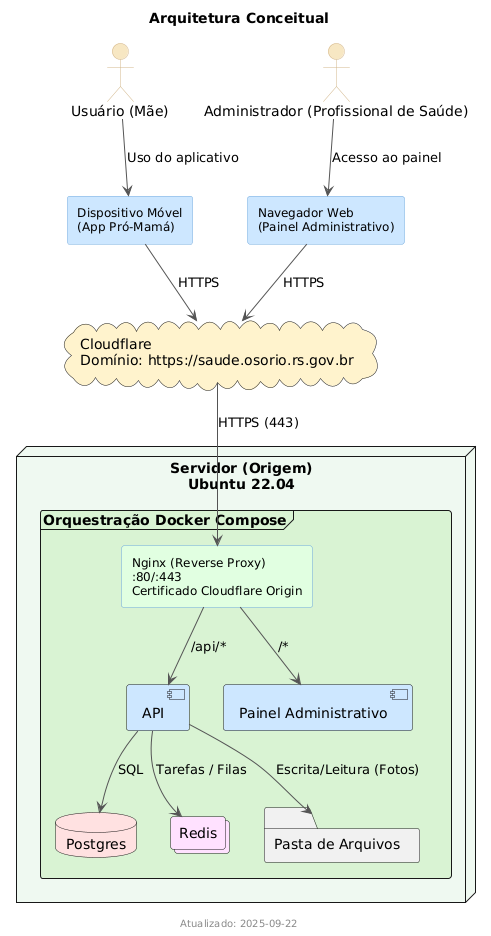
\includegraphics[width=0.8\textwidth]{imagens/promamamacro.png}
\caption{Visão geral dos componentes e interações do sistema Pró-Mamá.\\\small Fonte: Autoria Própria.}
\label{fig:macro-promama}
\end{figure}
\subsection{Codificação dos Componentes}

Após a definição dos módulos do sistema, procedeu-se à escolha de padrões de desenvolvimento que pudessem ser aplicados de forma consistente tanto na \emph{API} quanto no Painel Administrativo. O objetivo foi estabelecer uma estrutura de código que favorecesse a compreensão, manutenção e expansão por futuros desenvolvedores, independentemente da familiaridade prévia com o projeto.

Embora o \emph{JavaScript} não seja uma linguagem orientada a objetos de forma estrita, como o \emph{Java}, a adoção do \emph{TypeScript} permitiu incorporar recursos de tipagem estática e reforçar o paradigma de programação orientada a objetos. Essa abordagem contribuiu para maior clareza na definição de classes, \emph{interfaces} e contratos, além de facilitar a detecção precoce de erros durante o desenvolvimento.

Para a organização dos arquivos e módulos, foi adotada a arquitetura \emph{Hexagonal} (\emph{Ports and Adapters}), que promove o desacoplamento entre o núcleo da aplicação e suas \emph{interfaces} externas. Essa decisão está alinhada ao conceito de "Arquitetura Gritante" descrito por \citeonline{archlimpaunclebob}, segundo o qual a estrutura do código deve refletir o domínio do negócio, permitindo que qualquer desenvolvedor identifique o propósito do sistema apenas ao analisar sua organização.

A implementação seguiu ainda princípios selecionados da metodologia SOLID, com destaque para:
\begin{itemize}
    \item \textbf{S} — Princípio da Responsabilidade Única (\emph{Single Responsibility Principle}): cada módulo ou classe deve possuir apenas uma responsabilidade, reduzindo acoplamentos desnecessários.
    \item \textbf{I} — Princípio da Segregação de \emph{Interface} (\emph{Interface Segregation Principle}): \emph{interfaces} específicas são preferíveis a \emph{interfaces} genéricas, evitando que clientes dependam de métodos que não utilizam.
    \item \textbf{D} — Princípio da Inversão de Dependência (\emph{Dependency Inversion Principle}): módulos de alto nível e baixo nível devem depender de abstrações, e não de implementações concretas.
\end{itemize}

A aplicação desses padrões e princípios resultou em um código mais modular, flexível e testável, características essenciais para a evolução contínua do sistema e para a integração de novos colaboradores. Na sequência, serão apresentadas as escolhas tecnológicas e as implementações específicas realizadas na \emph{API} e no Painel Administrativo do Pró-Mamá.

\subsubsection{Codificação da API}

A \emph{API} do Pró-Mamá foi desenvolvida no ecossistema \emph{Node.js}, utilizando o \emph{framework} \emph{Express} para a construção de aplicações \emph{web} e serviços \emph{RESTful}. O termo \emph{RESTful} refere-se a um estilo arquitetural para sistemas distribuídos que utiliza o protocolo HTTP e princípios como recursos identificáveis por URIs, operações padronizadas (\emph{GET}, \emph{POST}, \emph{PUT}, \emph{DELETE}) e comunicação sem estado \cite{REFERENCIA_RESTFUL}. Essa abordagem é amplamente adotada para integração entre sistemas e facilita a interoperabilidade.

Para a documentação, adotou-se a especificação \emph{OpenAPI} por meio da ferramenta \emph{Swagger} \citeonline{swaggerdocs}, que permite a geração automática de documentação interativa e a validação das rotas diretamente pela \emph{interface} \emph{Swagger UI}. Essa prática assegura que a documentação permaneça sincronizada com o código-fonte, reduzindo a necessidade de manutenção manual.

O gerenciamento de dependências internas foi estruturado com a biblioteca \emph{awilix} \citeonline{awilixdocs}, que implementa o padrão de Injeção de Dependência (\emph{Dependency Injection}). A Injeção de Dependência é um padrão de projeto que consiste em fornecer a um componente as suas dependências externas por meio de abstrações, em vez de criá-las internamente, promovendo o desacoplamento e facilitando testes e manutenção \cite{REFERENCIA_DI}.

A organização da estrutura de pastas da \emph{API} seguiu uma divisão lógica, conforme a Tabela~\ref{tab:pastas_api}, separando responsabilidades e favorecendo a clareza arquitetural.

\begin{table}[H]
\centering
\caption{Estrutura de pastas da API e responsabilidades}
\label{tab:pastas_api}
\begin{tabular}{|l|p{10cm}|}
\hline
\textbf{Pasta} & \textbf{Responsabilidade} \\ \hline
\texttt{app} & Contém a configuração principal da aplicação, incluindo inicialização de serviços e carregamento de módulos. \\ \hline
\texttt{domain} & Implementa as regras de negócio e entidades centrais do sistema, isoladas de detalhes técnicos. \\ \hline
\texttt{infra} & Gerencia recursos de infraestrutura, como acesso a banco de dados e provedores (\emph{e-mail}, notificações). \\ \hline
\texttt{interfaces} & Define contratos e adaptadores para comunicação entre o núcleo da aplicação e componentes externos. \\ \hline
\texttt{jobs} & Armazena tarefas agendadas e processos assíncronos executados periodicamente. \\ \hline
\end{tabular}
\end{table}

Essa organização modular contribui para a manutenção evolutiva e a escalabilidade da solução. A estrutura estabelecida na \emph{API} serviu como base para o desenvolvimento do Painel Administrativo, que será detalhado na subseção seguinte.

\subsection{Codificação do Painel Administrativo}

O Painel Administrativo do Pró-Mamá foi desenvolvido como uma \emph{Single Page Application} (SPA). Uma SPA é uma aplicação \emph{web} que carrega uma única página HTML e atualiza dinamicamente o conteúdo conforme o usuário interage com a \emph{interface}, sem a necessidade de recarregar a página inteira \cite{REFERENCIA_SPA}. 

Essa abordagem proporciona uma experiência de uso mais fluida e responsiva, além de reduzir o tempo de carregamento entre páginas. No contexto do projeto, a escolha por uma SPA favorece a integração com a \emph{API} e permite que as funcionalidades administrativas sejam acessadas de forma contínua, sem interrupções na navegação.

Para a implementação, foi utilizada a biblioteca \emph{React.js}, amplamente adotada para construção de \emph{interfaces} de usuário baseadas em componentes \cite{REFERENCIA_REACT}. Essa arquitetura facilita a reutilização de elementos visuais e a manutenção do código, características essenciais para um projeto que poderá ser expandido por diferentes colaboradores ao longo do tempo.

A estrutura de pastas do Painel Administrativo foi adaptada da arquitetura utilizada na \emph{API}, considerando as necessidades específicas do \emph{frontend}. A Tabela~\ref{tab:pastas_painel} apresenta a organização adotada.

\begin{table}[H]
\centering
\caption{Estrutura de pastas do Painel Administrativo e responsabilidades}
\label{tab:pastas_painel}
\begin{tabular}{|l|p{10cm}|}
\hline
\textbf{Pasta} & \textbf{Responsabilidade} \\ \hline
\texttt{assets} & Contém arquivos estáticos como imagens, ícones e folhas de estilo globais. \\ \hline
\texttt{components} & Implementa componentes visuais reutilizáveis da interface (\emph{UI}). \\ \hline
\texttt{contexts} & Define contextos globais para gerenciamento de estado compartilhado entre componentes. \\ \hline
\texttt{global} & Armazena configurações e estilos globais aplicados em toda a aplicação. \\ \hline
\texttt{guards} & Implementa mecanismos de proteção de rotas, como verificação de autenticação. \\ \hline
\texttt{infra} & Gerencia integrações com serviços externos e recursos de infraestrutura do \emph{frontend}. \\ \hline
\texttt{domain} & Contém entidades e regras de negócio aplicadas no lado cliente. \\ \hline
\texttt{pages} & Agrupa as páginas principais da aplicação, cada uma representando uma rota distinta. \\ \hline
\texttt{providers} & Configura provedores de serviços e bibliotecas utilizadas globalmente. \\ \hline
\texttt{routes} & Define o mapeamento das rotas da aplicação e sua associação com componentes. \\ \hline
\end{tabular}
\end{table}

Para o gerenciamento de rotas, foi utilizada a biblioteca \emph{react-router-dom} \cite{REFERENCIA_ROUTER}, que permite definir caminhos e componentes associados, além de oferecer recursos para navegação programática e proteção de rotas. Essa escolha garante maior controle sobre a navegação interna da SPA e facilita a implementação de fluxos condicionais, como autenticação e autorização.

O processo de construção e otimização do Painel Administrativo foi realizado com o \emph{Vite} \cite{REFERENCIA_VITE}, uma ferramenta moderna de empacotamento e desenvolvimento que oferece inicialização rápida do servidor e atualização instantânea durante o desenvolvimento. Essa característica contribuiu para maior produtividade da equipe e para um ciclo de desenvolvimento mais ágil.

A adoção dessa arquitetura e conjunto de ferramentas assegura que o Painel Administrativo mantenha sintonia com a \emph{API}, tanto em organização quanto em práticas de desenvolvimento, favorecendo a manutenção e evolução conjunta das duas camadas do sistema.
